%\documentclass[a4paper,twocolumn]{article} % Document type

\documentclass[a4paper,12pt,oneside,onecolumn]{article} % Document type

\usepackage[left=1.0in, right=1.0in, top=1.0in, bottom=1.0in]{geometry}

\ifx\pdfoutput\undefined
    %Use old Latex if PDFLatex does not work
   \usepackage[dvips]{graphicx}% To get graphics working
   \DeclareGraphicsExtensions{.eps} % Encapsulated PostScript
 \else
    %Use PDFLatex
   \usepackage[pdftex]{graphicx}% To get graphics working
   \DeclareGraphicsExtensions{.pdf,.jpg,.png,.mps} % Portable Document Format, Joint Photographic Experts Group, Portable Network Graphics, MetaPost
   \pdfcompresslevel=9
\fi

\usepackage{amsmath,amssymb}   % Contains mathematical symbols
\usepackage[ansinew]{inputenc} % Input encoding, identical to Windows 1252
\usepackage[english]{babel}    % Language
\usepackage[square,numbers]{natbib}     %Nice numbered citations
\bibliographystyle{plainnat}            %Sorted bibliography
\usepackage{graphicx}
\usepackage{float}
\graphicspath{{fig/}}


\begin{document}               % Begins the document

\title{Homework 3 in EL2450 Hybrid and Embedded Control Systems}
\author{
  Alexander Ramm \\ 931005 \\ aleram@kth.se 
  \and 
  Filip Stenbeck \\ 930702 \\ fstenb@kth.se
  \and
  Gabriel Andersson Santiago \\ 910706 \\ gabras@kth.se
  \and
  Anders Levin
  }
%\date{2010-10-10}             % If you want to set the date yourself.

\maketitle                     % Generates the title




%%%%%%%%%%%%%%%%%%%%%%%%%%%%%%%%%%%%%%%%%%%%%%%%%%%%%%%%%%%%%%%%%%%%%%%%%%%%%%%%%%%
% Instructions regarding the report
%%%%%%%%%%%%%%%%%%%%%%%%%%%%%%%%%%%%%%%%%%%%%%%%%%%%%%%%%%%%%%%%%%%%%%%%%%%%%%%%%%%

\section*{Instructions and Help}

\textbf{Please remove this part and the sample references before submitting your homework.}

Read the general homework instructions available on the course homepage before starting to write the report.

Here are some additional guidelines how to write a homework report.
\begin{itemize}
 \item Fill in name and personal number of all group members.
 \item Do not copy the task descriptions and use the structure below.
 \item Do not include code unless the task explicitly states so.
 \item Motivate your answers well and how you derived them, but be concise.
 \item The number of points is not necessarily related to much you need to write for task.
 \item Put references in the end if any.
 \item Do not include plots from the Simulink scope (color on black background) but export the data to Matlab for plotting.
 \item Include graphics directly in the text and not in a Figure environment, as you normally would. That makes it easier to correct the report.
 \item There is plenty of material available how to use Latex. Use a search engine of your choice to learn more.
\end{itemize}

Here are some examples how to use Latex:
\begin{itemize}
 \item An equation with a reference \eqref{eq_sample} to it
 \begin{equation}
  \dot{x} = \frac{3}{4} x. \label{eq_sample}
 \end{equation}
 \item A multi-line equations with a reference to it
 \begin{align*}
  \hat{x} &= x - y\\
  \alpha &= x + \gamma.
 \end{align*}
 \item An equation in text: $\Phi = \int\limits_{0}^{h} \mathrm{e}^{A\tau} d \tau$.
 \item An image
 \begin{center}
  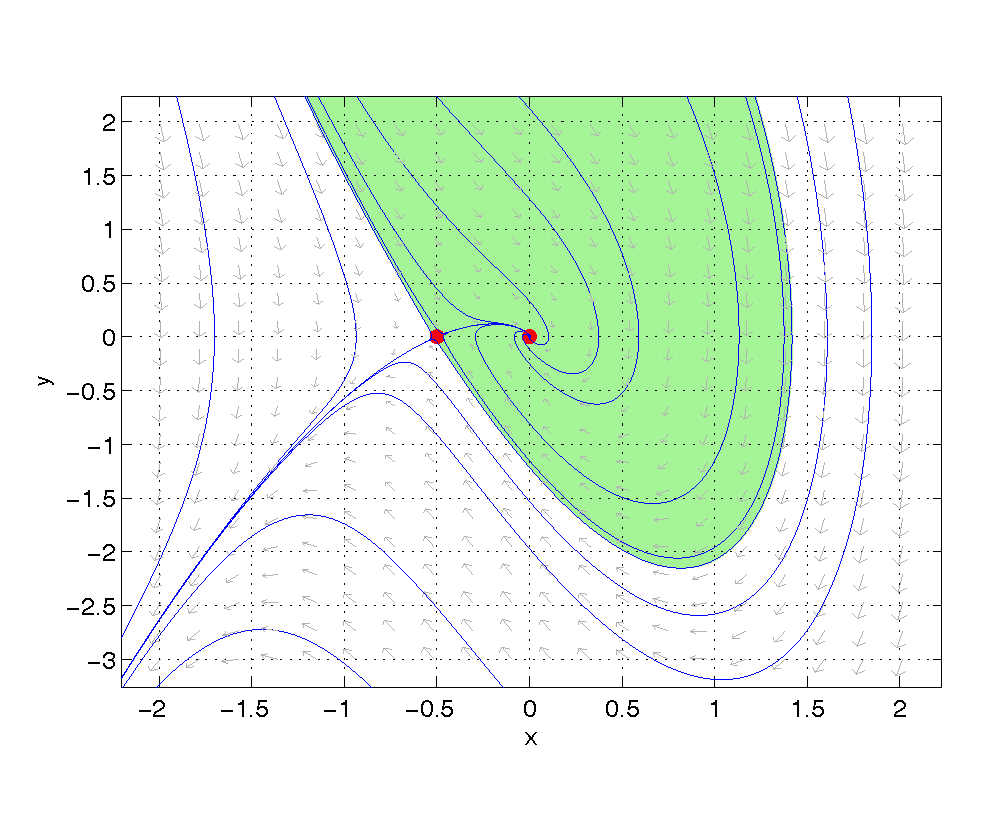
\includegraphics[width = 0.8\textwidth]{Phase_portrait_with_regionmark}
 \end{center}
 \item A table
 
 \begin{tabular}{@{\vrule height 10.5pt depth4pt  width0pt}|c|c|c|c|}
    \hline
     $-2.46$ & $0$ & $-1.73$ & $0$ \\ \hline
     $0$ & $-2.553$ & $0$ & $2.774$ \\ \hline
     $0$ & $6.172$ & $-10$ & $7.333$ \\ \hline
     $1.767$ & $-0.357$ & $5.714$ & $-6.074$ \\ \hline
  \end{tabular}
  \item A citation \cite{Oetiker:2008:TheNotSoShortIntroductiontoLaTeXe}
  \item Display something exactly as it is written: \verb|\frac{1}{2}_|
  \item Basic formating: \textbf{bold}, \textit{italics}, \texttt{typewriter}
\end{itemize}



\section*{Task 1}

\begin{equation}
u_r = \frac{2^{u_{\omega} + u_{\psi}}}{2} = u_w + \frac{u_{Psi}}{2}
\end{equation}
\begin{equation}
u_l = u_\omega - \frac{u_\Psi}{2}
\end{equation}

\section*{Task 2}

By calculating the mean value of $\dot{x}$ from the data in \emph{Forward.cvs} \emph{R} could be estimated with equation \eqref{xdot}
\begin{equation}
\dot{x} = R*u_\omega*cos(\theta) \label{xdot}
\end{equation}
\\
By calculating the mean value of $\dot{\theta}$ from the data in \emph{Rotate.cvs} \emph{L} could be estimated with equation \eqref{thetadot}
\begin{equation}
\dot{\theta} = \frac{R}{L}u_\Psi\label{thetadot}
\end{equation}
\\
The estimated values are
\begin{center}
	\begin{tabular}{| c | c |}
	\hline
	R & L \\ \hline
	111 & 111 \\ \hline
	
	\end{tabular}
\end{center}

\section*{Task 3}

$\dot{\theta} = R/L u_\psi$ won't be asymptotically stable due to that the output signal will oscillate with constant amplitude after a set time. It will not have Zeno behaviour due there is no finite time limit when the ouutput signal is stable. 


\section*{Task 4}

The system is asymptotically stable due to that the output signal will constantly converge to the desired value. Though by doing this will quicker and quicker reactions from the controller which will not be possible in real life. The system does not exhibit Zeno behaviour since the control signal will always have a value and it does not stabilize within a finite time. 


\section*{Task 5}

The system is stable but not asymptotically stable and therefore does also not exhibit Zeno behaviour. We see that the system is not asymptotically stable due to that the output signal does not converge to the desired value but will oscillate with a constant amplitude after infinite time.
\section*{Task 6}

The discretized system can be seen in Equations \eqref{dXdot},\eqref{dYdot} and\eqref{dPdot}
\begin{equation}
\frac{z-1}{T_s} x[k] = Ru_\omega[k] cos(\theta[k])\label{dXdot}
\end{equation}

\begin{equation}
\frac{z-1}{T_s} y[k] = Ru_\omega[k] sin(\theta[k]) \label{dYdot}
\end{equation}

\begin{equation}
\frac{z-1}{T_s} \theta[k] = \frac{R}{L}u_\Psi[k]\label{dPdot}
\end{equation}


\section*{Task 7}

With euler forward method we have that
\begin{equation*}
\theta[h]\approx \theta[k]+\dot{\theta}[k]\tau_s
\end{equation*}
We have $\dot{\theta}$ from equation (3) and control signal $u_\Psi$ in the assignment. This give the following equation for the system.
\begin{equation*}
\theta[k+h]\approx  \frac{R K_\Psi \tau_s(\theta^R-\theta[k])}{L}+\theta[k]
\end{equation*}

\begin{equation*}
\theta[k+h]\approx  (1-\frac{R K_\Psi \tau_s)}{L})\theta[k]+\frac{R K_\Psi \tau_s)}{L}\theta^R
\end{equation*}
This is stable i the absolute value of the eigenvalues are less than 1 for the $\Phi$ matrix. The eigenvalue is
\begin{equation*}
\lambda = |1-\frac{R K_\Psi \tau_s)}{L}|<1
\end{equation*}
This gives the the upper/lower boundary of $0<K_\Psi<\frac{2L}{R\tau_s}$. 

\section*{Task 8}

It is not possible to reach the goal angle due to we only have a proportional controller and therefore always have a small static error.

K = 0.7*L/R
\begin{figure}[H]
\begin{center}	
  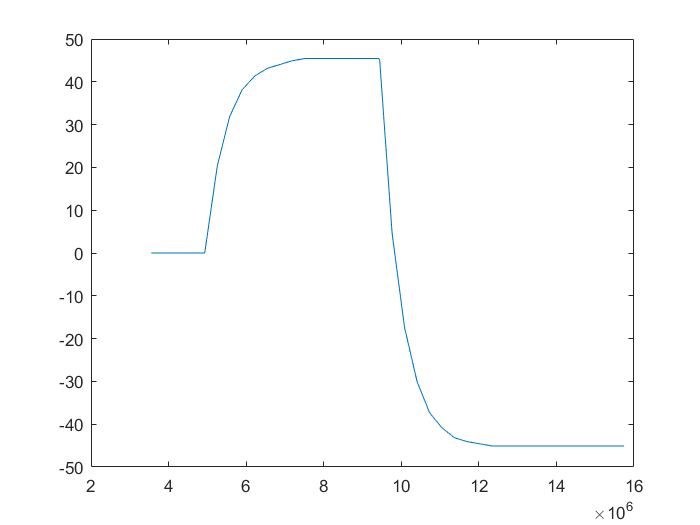
\includegraphics[width = 0.8\textwidth]{task8.png}
 \end{center}
\end{figure}
\section*{Task 9}
With euler forward method we have that for the x variable
\begin{equation*}
x[h]\approx x[k]+\dot{x}[k]\tau_s
\end{equation*}
We have $\dot{x}$ from equation (3) and control signal $u_\omega$.
\begin{equation*}
u_\omega [k] = K_{\omega} cos(\theta [k])(x_0 - x[k])+K_{\omega}sin(\theta [k]) (y_0-y[k])
\end{equation*}
\begin{equation*}
\dot{x[k]} = R u_\omega [k] cos(\theta[k])
\end{equation*}
\begin{equation*}
x[k+h]\approx  (1-K_\omega\tau_sRcos^2(\theta[k]))x[k]+K_1+\Gamma y[k]
\end{equation*}
Where $K_1$ a constant of how $x[k+h]$ depends on $x_0, y_0$ and $\Gamma$ is how it depends on the position i y direction $y[k]$. Assuming that $y[k]$ could be considered as an input signal we have stability if the absolute value of the eigenvalues in the stability equation is less than $1$.
\begin{equation*}
|\lambda |=|1-K_\omega\tau_sRcos^2(\theta[k])|<1
\end{equation*}
This gives the the upper/lower boundary of $0<K_\omega<\frac{2}{R\tau_s}$ since the minumum upper boundary is found when $cos^2(\theta[k])=1$.\\\\
If the controller is analysed in the y direction the following eigenvalues are obtained.
\begin{equation*}
|\lambda |=|1-K_\omega\tau_sRsin^2(\theta[k])|<1
\end{equation*} And since the maximum of $sin^2(\theta[k])=cos^2(\theta[k])=1$ gives the same upper and lower bounds.


\section*{Task 10}
K = 5
In the general case no due to the direction of the robot is not lined up with the point it wants to go to. 
\begin{figure}[H]
\begin{center}	
  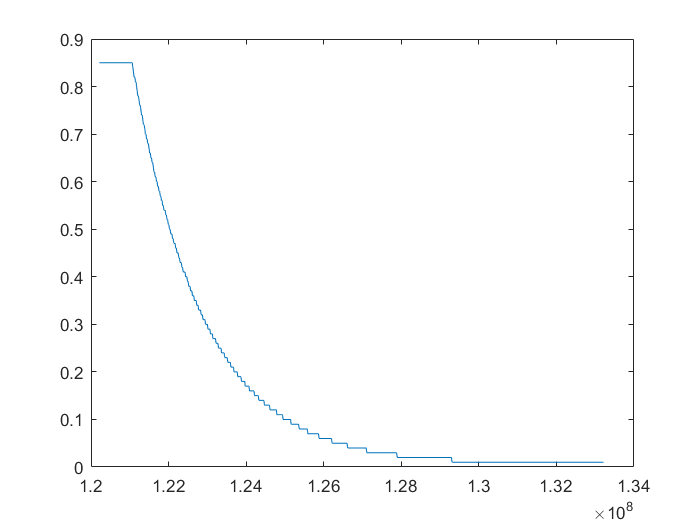
\includegraphics[width = 0.8\textwidth]{task10.png}
 \end{center}
\end{figure}

\section*{Task 11}

\begin{figure}[H]
\begin{center}	
  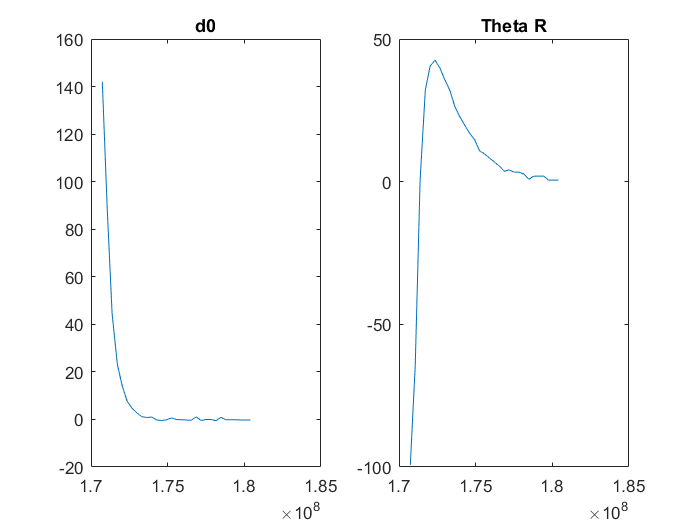
\includegraphics[width = 0.8\textwidth]{task11.png}
 \end{center}
\end{figure}

\section*{Task 12}
This section is very similar to task 9 whilst we have a slightly different controller thus this will not change the poles of the controller. Again the position approximated with euler forward. 
\begin{equation*}
x[h]\approx x[k]+\dot{x}[k]\tau_s
\end{equation*}
We have $\dot{x}$ from equation (3) and control signal $u_\omega$.
\begin{equation*}
u_\omega [k] = K_{\omega} cos(\theta [k])(x_g - x[k])+K_{\omega}sin(\theta [k]) (y_g-y[k])
\end{equation*}
\begin{equation*}
\dot{x[k]} = R u_\omega [k] cos(\theta[k])
\end{equation*}
\begin{equation*}
x[k+h]\approx  (1-K_\omega\tau_sRcos^2(\theta[k]))x[k]+K_1+\Gamma y[k]
\end{equation*}
Where $K_1$ a constant of how $x[k+h]$ depends on $x_g, y_g$ and $\Gamma$ is how it depends on the position i y direction $y[k]$. Assuming that $y[k]$ could be considered as an input signal we have stability if the absolute value of the eigenvalues in the stability equation is less than $1$.
\begin{equation*}
|\lambda |=|1-K_\omega\tau_sRcos^2(\theta[k])|<1
\end{equation*}
This gives the the upper/lower boundary of $0<K_\omega<\frac{2}{R\tau_s}$ since the minumum upper boundary is found when $cos^2(\theta[k])=1$. This is just like the controller in task 9 but we control to a different position. \\\\
If the controller is analysed in the y direction the following eigenvalues are obtained.
\begin{equation*}
|\lambda |=|1-K_\omega\tau_sRsin^2(\theta[k])|<1
\end{equation*} And since the maximum of $sin^2(\theta[k])=cos^2(\theta[k])=1$ gives the same upper and lower bounds.
\section*{Task 13}
K = 30
\begin{figure}[H]
\begin{center}	
  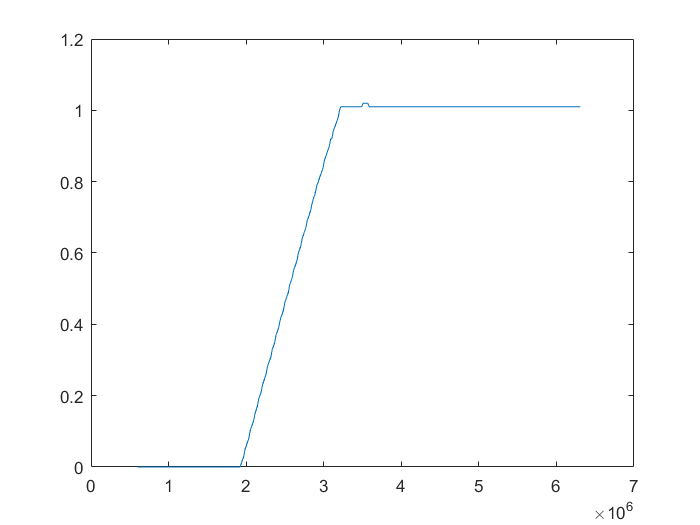
\includegraphics[width = 0.8\textwidth]{task13.png}
 \end{center}
\end{figure}

\section*{Task 14}

Solution to the task

\section*{Task 15}

Solution to the task

\section*{Task 16}

Solution to the task

\section*{Task 17}

Solution to the task

\section*{Task 18}

	$Q = \{Rotate,Line,Wait\}$\\
	$X = \mathbb{R}^3$\\
	$Init = (Rotation,(x0,y0,\theta0)$
	\\
	$f(Rotation,(x,y,\theta)) = (Ru_\omega*cos(\theta),Ru_\omega*sin(\theta),\frac{R}{L}u_\Psi)$\\
	$f(Line,(x,y,\theta)) = (Ru_\omega*cos(\theta),Ru_\omega*sin(\theta),\frac{R}{L}u_\Psi)$\\
	$f(Wait,(x,y,\theta)) = (0,0,0)$\\
	\\
	$D(Rotation) = \{(x,y,\theta) \epsilon \mathbb{R}, -180 < \theta <= 180\}$\\
	$D(Line) = \{(x,y,\theta) \epsilon \mathbb{R}, -180 < \theta <= 180\}$\\
	$D(Wait) = \{(x,y,\theta) \epsilon \mathbb{R}, -180 < \theta <= 180\}$\\
	\\
	$E = \{ (Rotation,line),(Line,Wait),(Line,Rotation),(Wait,Rotation)\}$\\\\
	$G(Rotation, Line) = \{(x,y,\theta) \epsilon \mathbb{R}: |\theta^R - \theta| < a, |x0 - x| < b, |y0 -y| < c\}$\\
	$G(Line, Rotation)=\{(x,y,\theta) \epsilon \mathbb{R}: |xg - x|<d,|yg -y|<e\}$\\\\	
	$R((Rotation, Line), ((x,y,\theta) \epsilon \mathbb{R}))=$ 
	$R((Line, Wait), ((x,y,\theta) \epsilon \mathbb{R}))=$\\
	$=R((Line, Rotation), ((x,y,\theta) \epsilon \mathbb{R}))=$
	$R((Wait, Rotation), ((x,y,\theta) \epsilon \mathbb{R}))=$\\$\{(x,y,\theta) \epsilon \mathbb{R}\}$\\


\section*{Task 19}

Solution to the task

\section*{Task 20}

Solution to the task

\section*{Task 21}

Solution to the task

\section*{Task 22}

Solution to the task



%%%%%%%%%%%%%%%%%%%%%%%%%%%%%%%%%%%%%%%%%%%%%%%%%%%%%%%%%%%%%%%%%%%%%%%%%%%%%%%%%%%
% The bibliography
%%%%%%%%%%%%%%%%%%%%%%%%%%%%%%%%%%%%%%%%%%%%%%%%%%%%%%%%%%%%%%%%%%%%%%%%%%%%%%%%%%%
%\bibliography{Bibliography_template} %Read the bibliography from a separate file

\begin{thebibliography}{99}
\bibitem[Khalil(2002)]{Khalil:2002:Nonlinear-systems:vh}
Hassan~K Khalil.
\newblock \emph{Nonlinear systems}.
\newblock Prentice Hall, Upper Saddle river, 3. edition, 2002.
\newblock ISBN 0-13-067389-7.

\bibitem[Oetiker et~al.(2008)Oetiker, Partl, Hyna, and
  Schlegl]{Oetiker:2008:TheNotSoShortIntroductiontoLaTeXe}
Tobias Oetiker, Hubert Partl, Irene Hyna, and Elisabeth Schlegl.
\newblock \emph{The Not So Short Introduction to \LaTeXe}.
\newblock Oetiker, OETIKER+PARTNER AG, Aarweg 15, 4600 Olten, Switzerland,
  2008.
\newblock http://www.ctan.org/info/lshort/.

\bibitem[Sastry(1999)]{Sastry:1999:Nonlinear-systems:-analysis-stability-and-c%
ontrol:xr}
Shankar Sastry.
\newblock \emph{Nonlinear systems: analysis, stability, and control},
  volume~10.
\newblock Springer, New York, N.Y., 1999.
\newblock ISBN 0-387-98513-1.
\end{thebibliography}


\end{document}      % End of the document
